
% %%%%%%%%%%%%%%%%%%%%%%%%%%%%%%%%%%%%%%%%%%%%%%%%%%%%%%%%%%%%%%%%%%%%%%%%%%%%%%%
% \begin{frame}{Improving Robustness with Lipschitz Regularization}
% %%%%%%%%%%%%%%%%%%%%%%%%%%%%%%%%%%%%%%%%%%%%%%%%%%%%%%%%%%%%%%%%%%%%%%%%%%%%%%%
%
%   \citet{farnia2018generalizable} have shown that the adversarial generalization error depends on the Lipschitz constant of the network. 
%   \begin{itemize}
%     \item[$\Rightarrow$] Reducing the Lipschitz constant of the Neural Network will improve robustness against adversarial attacks
%   \end{itemize}
%
%   % $\Rightarrow$ Adversarial test error can be improved by reducing the Lipschitz regularization in addition to adversarial training, we propose the following:
%
% \end{frame}


% %%%%%%%%%%%%%%%%%%%%%%%%%%%%%%%%%%%%%%%%%%%%%%%%%%%%%%%%%%%%%%%%%%%%%%%%%%%%%%%
% \begin{frame}{Lipschitz constant of a Neural Network}
% %%%%%%%%%%%%%%%%%%%%%%%%%%%%%%%%%%%%%%%%%%%%%%%%%%%%%%%%%%%%%%%%%%%%%%%%%%%%%%%
%   The \textbf{Lipschitz constant} w.r.t $\ell_2$ of a function is the smallest constant K such that:
%   \begin{equation}
%     \norm{f(\xvec) - f(\yvec)}_2 \leq K \norm{\xvec - \yvec}_2
%   \end{equation}
%   Let us denote $\lip(f) = K$ or that $f$ is $K$-Lipschitz.
%
%   The Lipschitz constant of the composition of multiple functions can be upper bounded by the product of the Lipschitz constant of each function.
%
%   Remarks:
%   \begin{itemize}
%     \small
%     \item[$\bullet$] For a linear function, the Lipschitz constant also corresponds to the maximal singular value. 
%     \item[$\bullet$] Usual non-linear functions used in Neural Networks (\eg ReLU) are 1-Lipschitz
%   \end{itemize}
%
%   Therefore, we can upper bound the Lipschitz constant of a Neural Network $N$ as follows:
%   \begin{equation}
%     \lip(N_\Omega) \leq \prod_{i=0}^p \lip(\phi_{\Wmat_i, \bvec_i}) = \prod_{i=0}^p \sigma_1(\Wmat_i)
%   \end{equation}
%
%   \begin{itemize}
%     \item[$\Rightarrow$] This bound is hard to compute
%   \end{itemize}
%  
% \end{frame}


% %%%%%%%%%%%%%%%%%%%%%%%%%%%%%%%%%%%%%%%%%%%%%%%%%%%%%%%%%%%%%%%%%%%%%%%%%%%%%%%
% \begin{frame}{Convolution as matrix-multiplication}
% %%%%%%%%%%%%%%%%%%%%%%%%%%%%%%%%%%%%%%%%%%%%%%%%%%%%%%%%%%%%%%%%%%%%%%%%%%%%%%%
%
%   A discrete convolution between a signal $\xvec$ and a kernel $\kvec$ can be expressed as a product between the vectorization of $\xvec$ and a doubly-block Toeplitz matrix $\Mmat$, whose coefficients have been chosen to match the convolution $\xvec * \kvec$.
%
%   {\color{red}{TO CHANGE}}
%
%   \begin{figure}
%     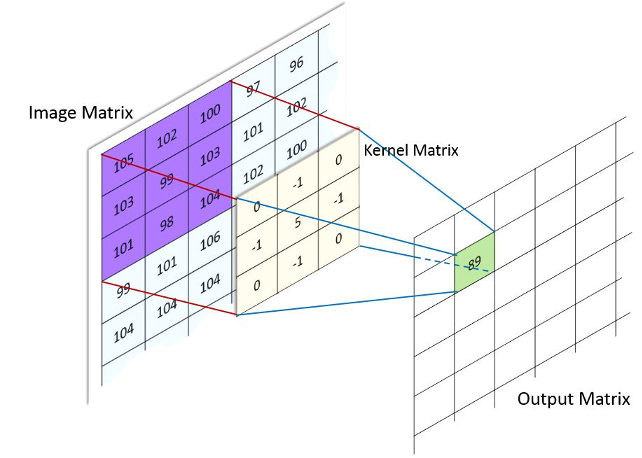
\includegraphics[width=0.5\textwidth]{images/convolution.png}
%     \caption*{Convolution between a 2-dimensional image and a 2 dimensional kernel}
%   \end{figure}
%
%   The convolution is equivalent to a matrix-vector product between a \textbf{doubly-block Toeplitz matrix} and the vectorize image. 
%
% \end{frame}





% %%%%%%%%%%%%%%%%%%%%%%%%%%%%%%%%%%%%%%%%%%%%%%%%%%%%%%%%%%%%%%%%%%%%%%%%%%%%%%%
% \begin{frame}{Generating functions of Toeplitz and block Toeplitz matrices}
% %%%%%%%%%%%%%%%%%%%%%%%%%%%%%%%%%%%%%%%%%%%%%%%%%%%%%%%%%%%%%%%%%%%%%%%%%%%%%%%
%
%   \begin{itemize}
%     \item[$\bullet$] <1-> A $n\times n$ Toeplitz matrix $\Amat$ is \orangebold{fully determined by a two-sided sequence of scalars}:  $\{\asf_h\}_{h \in \{-n+1, \dots, n-1\}}$
%     \item[$\bullet$] <2-> A $nm \times nm$ block Toeplitz matrix $\Bmat$ is \orangebold{fully determined by a two-sided sequence of blocks}: $\{\Bsf_h\}_{h \in \{-n+1,\dots,n-1\}}$ where each block $\Bsf_h$ is a $m \times m$ matrix 
%    \end{itemize}
%     
%   % A $n\times n$ Toeplitz matrix $\Amat$ is fully determined by a two-sided sequence of scalars: $\{\asf_h\}_{h \in \seqsetN}$, whereas a $nm \times nm$ block Toeplitz matrix $\Bmat$ is fully determined by a two-sided sequence of blocks $\{\Bsf_h\}_{h \in \seqsetN}$, where $\seqsetN = \{-n+1,\dots, n-1 \}$ and where each block $\Bsf_h$ is a $m \times m$ matrix.  
%
%   \only<1>{
%     \begin{equation}
% 	\Amat = \begin{pmatrix}
% 	  \asf_0 & \asf_{1} & \cdots & \asf_{n-1} \\ \vspace{0.1cm}
% 	  \asf_{-1} & \asf_0 & \ddots & \vdots \\ \vspace{0.3cm}
% 	  \vdots & \ddots & \asf_{0} & \asf_{1} \\ 
% 	  \asf_{-n+1} & \cdots  & \asf_{-1}    & \asf_0 
% 	\end{pmatrix} \phantom{\quad \quad 
% 	\Bmat =\begin{pmatrix}
% 	  \Bsf_0 & \Bsf_{1} & \cdots & \Bsf_{n-1} \\ \vspace{0.1cm}
% 	  \Bsf_{-1} & \Bsf_0 & \ddots & \vdots \\ \vspace{0.3cm}
% 	 \vdots & \ddots & \Bsf_0 & \Bsf_{1} \\ 
% 	\Bsf_{-n+1} & \cdots  & \Bsf_{-1}    & \Bsf_0 
%       \end{pmatrix}.}
%     \end{equation}
%     \begin{minipage}{0.52\textwidth}
%       \centering
%       \footnotesize Toeplitz matrix.
%     \end{minipage}
%   }
%
%   \only<2>{
%     \begin{equation}
% 	\Amat = \begin{pmatrix}
% 	  \asf_0 & \asf_{1} & \cdots & \asf_{n-1} \\ \vspace{0.1cm}
% 	  \asf_{-1} & \asf_0 & \ddots & \vdots \\ \vspace{0.3cm}
% 	  \vdots & \ddots & \asf_{0} & \asf_{1} \\ 
% 	  \asf_{-n+1} & \cdots  & \asf_{-1}    & \asf_0 
% 	\end{pmatrix} \quad \quad 
% 	\Bmat =\begin{pmatrix}
% 	  \Bsf_0 & \Bsf_{1} & \cdots & \Bsf_{n-1} \\ \vspace{0.1cm}
% 	  \Bsf_{-1} & \Bsf_0 & \ddots & \vdots \\ \vspace{0.3cm}
% 	 \vdots & \ddots & \Bsf_0 & \Bsf_{1} \\ 
% 	\Bsf_{-n+1} & \cdots  & \Bsf_{-1}    & \Bsf_0 
% 	\end{pmatrix}.
%     \end{equation}
%     \begin{minipage}{0.52\textwidth}
%       \centering
%       \footnotesize Toeplitz matrix.
%     \end{minipage}
%     \hfill
%     \begin{minipage}{0.41\textwidth}
%       \centering
%       \footnotesize Block Toeplitz matrix.
%     \end{minipage}
%   }
%
%   % with $\seqsetN = \{-n+1,    \dots, n-1 \}$
%
%   % We also write:
%   % \begin{equation}
%   %   \Amat = (\asf_{j-i})_{i, j \in \{0, \dots, n-1\}} \quad \quad
%   %   \Bmat = (\Bsf_{j-i})_{i, j \in \{0, \dots, n-1\}}
%   % \end{equation}
%
% \end{frame}



% %%%%%%%%%%%%%%%%%%%%%%%%%%%%%%%%%%%%%%%%%%%%%%%%%%%%%%%%%%%%%%%%%%%%%%%%%%%%%%%
% \begin{frame}{Generating functions of Toeplitz and block Toeplitz matrices}
% %%%%%%%%%%%%%%%%%%%%%%%%%%%%%%%%%%%%%%%%%%%%%%%%%%%%%%%%%%%%%%%%%%%%%%%%%%%%%%%
%
%   The matrices $\Amat$ and $\Bmat$ can be written in matrix form as follows:
%   \begin{equation}
%     \Amat = (\orange{\asf_{j-i}})_{i, j \in [n-1]} \quad \quad
%     \Bmat = (\orange{\Bsf_{j-i}})_{i, j \in [n-1]}
%   \end{equation}
%
%   \pause
%   Let us define a complex-valued function and a matrix-valued function which are the \orangebold{inverse Fourier Transform} of the sequences $\{\asf_h\}_{h \in N}$ and $\{\Bsf\}_{h \in N}$ as follows:
%   \begin{equation}
%     f(\omega) = \sum_{h \in N} \orange{\asf_h} e^{\ci h \omega} \quad \quad G(\omega) = \sum_{h \in N} \orange{\Bsf_h} e^{\ci h \omega} 
%   \end{equation}
%
%   \pause
%   One can recover these two sequences using the standard \orangebold{Fourier transform}:
%   \begin{equation}
%     \asf_\seqidx = \frac{1}{2\pi} \int_0^{2\pi} e^{-\ci \seqidx \omega} f(\omega) d\omega \quad \quad \Bsf_\seqidx = \frac{1}{2\pi} \int_0^{2\pi} e^{-\ci \seqidx \omega} G(\omega) d\omega .
%   \end{equation}
%
%   \pause
%   Therefore, we can express the matrices $\Amat$ and $\Bmat$ as follows
%   % by taking the Fourier transform of the function $f$ and $G$ respectively:
%   \begin{equation}
%     \Amat = \left( \frac{1}{2\pi} \int_0^{2\pi} e^{-\ci h \omega} \orange{f(\omega)} d\omega \right)_{i, j \in [n-1]} \quad 
%     \Bmat = \left( \frac{1}{2\pi} \int_0^{2\pi} e^{-\ci h \omega} \orange{G(\omega)} d\omega \right)_{i, j \in [n-1]}
%   \end{equation}
%
% \end{frame}



% %%%%%%%%%%%%%%%%%%%%%%%%%%%%%%%%%%%%%%%%%%%%%%%%%%%%%%%%%%%%%%%%%%%%%%%%%%%%%%%
% \begin{frame}{Empirical Results -- CIFAR-10 Dataset}
% %%%%%%%%%%%%%%%%%%%%%%%%%%%%%%%%%%%%%%%%%%%%%%%%%%%%%%%%%%%%%%%%%%%%%%%%%%%%%%%
%
%   {\color{red}{merge two slide CIFAR / imageNet}} 
%
%   \begin{block}{Dataset: CIFAR-10}
%   \begin{itemize}
%     \item 50K images
%     \item 10 classes
%   \end{itemize}
%   \end{block}
%
%   \begin{table}[t]
%     \centering
%       {\small
%       \begin{tabular}{lrrrr}
%       \toprule
%       & \textbf{Accuracy} & \textbf{PGD-$\ell_\infty$ 0.03} & \textbf{C\&W-$\ell_2$ 0.6} & \textbf{C\&W-$\ell_2$ 0.8} \\
%       \midrule
%       \textbf{Baseline} & $\mathbf{0.953}$ & $\phantom{.}0.000$ & $\phantom{.}0.002$ & $\phantom{.}0.000$ \\
%       \textbf{AT} & $\phantom{.}0.864$ & $\phantom{.}0.426$ & $\phantom{.}0.477$ & $\phantom{.}0.334$ \\
%       \textbf{AT+LipReg} & $\phantom{.}0.808$ & $\mathbf{0.457}$ & $\mathbf{0.547}$ & $\mathbf{0.438}$ \\
%       \midrule
%       \textbf{Diff} & $-0.056$ & $+0.031$ & $+0.07$ & $+0.104$ \\
%       \bottomrule
%       \end{tabular}%
%       }
%     \caption{This table shows the Accuracy under $\ell_2$ and $\ell_\infty$ attacks of CIFAR10 dataset. We use $\lambda$ equals to $0.008$.}
%     \label{tab:table_cifar10_robustness}%
%   \end{table}%
%
% \end{frame}
%
%
%
%
%
% %%%%%%%%%%%%%%%%%%%%%%%%%%%%%%%%%%%%%%%%%%%%%%%%%%%%%%%%%%%%%%%%%%%%%%%%%%%%%%%
% \begin{frame}{Empirical Results -- ImageNet Dataset}
% %%%%%%%%%%%%%%%%%%%%%%%%%%%%%%%%%%%%%%%%%%%%%%%%%%%%%%%%%%%%%%%%%%%%%%%%%%%%%%%
%
%   \begin{block}{Dataset: ImageNet}
%   \begin{itemize}
%     \item 1,2 millions images
%     \item 1000 classes
%   \end{itemize}
%   \end{block}
%
%   \begin{table}[htbp]
%     \centering
%      \begin{tabular}{lrrrr}
%      \toprule
%        & \multicolumn{1}{l}{\textbf{Accuracy}} & \multicolumn{1}{c}{\textbf{PGD-}$\ell_\infty$ 0.02} & \multicolumn{1}{l}{\textbf{C\&W-}$\ell_2$ 1} & \multicolumn{1}{l}{\textbf{C\&W-}$\ell_2$ 2} \\
%      \midrule
%      AT & 0.509 & 0.251 & 0.307 & 0.168 \\
%      AT+LipReg & \textbf{0.519} & \textbf{0.259} & \textbf{0.338} & \textbf{0.204} \\
%      \bottomrule
%      \end{tabular}%
%      \caption{This table shows the accuracy and accuracy under attack of ImageNet dataset with different training schemes. We compare Adversarial Training with the combination of Lipschitz regularization and Adversarial Training (\cite{madry2018towards}). We use $\lambda$  equal to $0.01$}
%   \end{table}%
%
% \end{frame}




% %%%%%%%%%%%%%%%%%%%%%%%%%%%%%%%%%%%%%%%%%%%%%%%%%%%%%%%%%%%%%%%%%%%%%%%%%%%%%%%
% \begin{frame}{Structured matrices for Deep Neural Networks}
% %%%%%%%%%%%%%%%%%%%%%%%%%%%%%%%%%%%%%%%%%%%%%%%%%%%%%%%%%%%%%%%%%%%%%%%%%%%%%%%
%
%   A $n \times n$ structured matrix can be represented with less than $n^2$ parameters.
%
%   \begin{figure}[ht]
%      \centering
%      \begin{subfigure}[t]{2.2cm}
% 	 \centering
% 	 \begin{equation}
% 	   \begin{pmatrix}
% 	     {\color{color1}{\absf}} &   &   &   \\
% 	     & {\color{color2}{\bbsf}} &   &   \\
% 	     &   & {\color{color3}{\cbsf}} &   \\
% 	     &   &   & {\color{color4}{\dbsf}}
% 	   \end{pmatrix}
% 	 \end{equation}
% 	 \caption*{\textbf{Diagonal}}
%      \end{subfigure}
%      \hspace{0.5cm}
%      \begin{subfigure}[t]{2.2cm}
% 	 \centering
% 	 \begin{equation}
% 	    \begin{pmatrix}
% 	      {\color{color1}{\absf}} & {\color{color2}{\bbsf}} & {\color{color3}{\cbsf}} & {\color{color4}{\dbsf}} \\
% 	      {\color{color6}{\ebsf}} & {\color{color1}{\absf}} & {\color{color2}{\bbsf}} & {\color{color3}{\cbsf}} \\
% 	      {\color{color7}{\fbsf}} & {\color{color6}{\ebsf}} & {\color{color1}{\absf}} & {\color{color2}{\bbsf}} \\
% 	      {\color{color8}{\gbsf}} & {\color{color7}{\fbsf}} & {\color{color6}{\ebsf}} & {\color{color1}{\absf}}
% 	    \end{pmatrix}
% 	 \end{equation}
% 	 \caption*{\textbf{Toeplitz}}
%      \end{subfigure}
%      \hspace{0.5cm}
%      \begin{subfigure}[t]{2.8cm}
% 	 \centering
% 	 \begin{equation}
% 	    \begin{pmatrix}
% 	      {\color{color1}{\absf}} & {\color{color1}{\absf}}^2 & {\color{color1}{\absf}}^3 & {\color{color1}{\absf}}^4 \\
% 	      {\color{color2}{\bbsf}} & {\color{color2}{\bbsf}}^2 & {\color{color2}{\bbsf}}^3 & {\color{color2}{\bbsf}}^4 \\
% 	      {\color{color3}{\cbsf}} & {\color{color3}{\cbsf}}^2 & {\color{color3}{\cbsf}}^3 & {\color{color3}{\cbsf}}^4 \\
% 	      {\color{color4}{\dbsf}} & {\color{color4}{\dbsf}}^2 & {\color{color4}{\dbsf}}^3 & {\color{color4}{\dbsf}}^4
% 	    \end{pmatrix}
% 	 \end{equation}
% 	 \caption*{\textbf{Vandermonde}}
%      \end{subfigure}
%   \end{figure}
%
%   In addition to offering a more compact representation, the structure of certain matrices can be leveraged to obtain better algorithms for matrix-vector product.
%
%   % $\Rightarrow$ We focus on structured matrices from the \textbf{Toeplitz family}. 
%
% \end{frame}


% %%%%%%%%%%%%%%%%%%%%%%%%%%%%%%%%%%%%%%%%%%%%%%%%%%%%%%%%%%%%%%%%%%%%%%%%%%%%%%%
% \begin{frame}{Focus on structured matrices from the Toeplitz family}
% %%%%%%%%%%%%%%%%%%%%%%%%%%%%%%%%%%%%%%%%%%%%%%%%%%%%%%%%%%%%%%%%%%%%%%%%%%%%%%%
%
%   More specifically: A Toeplitz matrix is a matrix with constant diagonal:
%   \vspace{0.6cm}
%
%   \begin{minipage}{0.3\textwidth}
%      \centering
%      \begin{equation}
% 	\begin{pmatrix}
% 	  {\color{color1}{\absf}} & {\color{color2}{\bbsf}} & {\color{color3}{\cbsf}} & {\color{color4}{\dbsf}} & {\color{color5}{\ebsf}} \\
% 	  {\color{color6}{\fbsf}} & {\color{color1}{\absf}} & {\color{color2}{\bbsf}} & {\color{color3}{\cbsf}} & {\color{color4}{\dbsf}} \\
% 	  {\color{color7}{\gbsf}} & {\color{color6}{\fbsf}} & {\color{color1}{\absf}} & {\color{color2}{\bbsf}} & {\color{color3}{\cbsf}} \\
% 	  {\color{color8}{\hbsf}} & {\color{color7}{\gbsf}} & {\color{color6}{\fbsf}} & {\color{color1}{\absf}} & {\color{color2}{\bbsf}} \\ 
% 	  {\color{color9}{\ibsf}} & {\color{color8}{\hbsf}} & {\color{color7}{\gbsf}} & {\color{color6}{\fbsf}} & {\color{color1}{\absf}}  
% 	\end{pmatrix}
%      \end{equation}
%   \end{minipage}
%   \hfill
%   \begin{minipage}{0.3\textwidth}
%     \vspace{0.5cm}
%     \centering
%     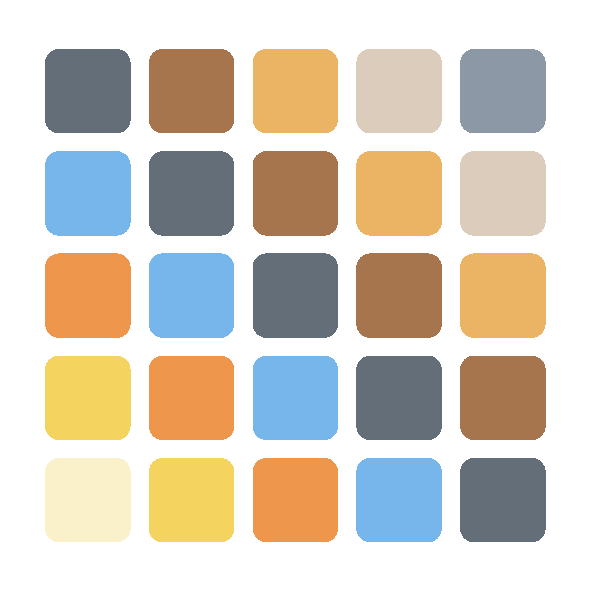
\includegraphics[scale=0.25]{images/toeplitz_v1.pdf}
%   \end{minipage}
%   \hfill
%   \begin{minipage}{0.3\textwidth}
%     \vspace{0.5cm}
%     \centering
%     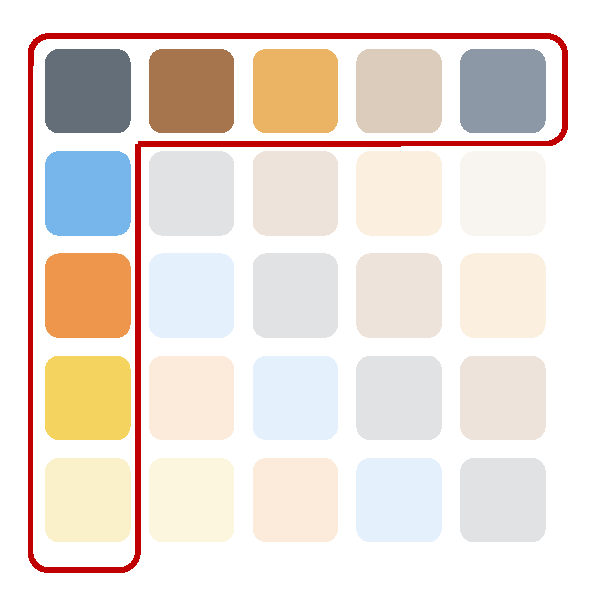
\includegraphics[scale=0.25]{images/toeplitz_v2.pdf}
%   \end{minipage}
%
%
%   \vspace{0.8cm}
%   $\Rightarrow$ A $n \times n$ Toeplitz matrix has $2n - 1$ unique values. 
%
% \end{frame}






% %%%%%%%%%%%%%%%%%%%%%%%%%%%%%%%%%%%%%%%%%%%%%%%%%%%%%%%%%%%%%%%%%%%%%%%%%%%%%%%
% \begin{frame}{Conclusion}
% %%%%%%%%%%%%%%%%%%%%%%%%%%%%%%%%%%%%%%%%%%%%%%%%%%%%%%%%%%%%%%%%%%%%%%%%%%%%%%%
%  
%   \begin{block}{Designing compact neural networks with structured matrices}
%   \begin{itemize}
%     \pause
%     \item[$\bullet$] We proposed the use of a matrix decomposition into diagonal and circulant matrices in Deep Learning settings
%     \pause
%     \item[$\bullet$] We proposed the use of a matrix decomposition into diagonal and circulant matrices in Deep Learning settings
%     \pause
%     \item[$\bullet$] We applied have applied this structure for large scale video classification
%     \pause
%     \item We showed that this method allows a good compression rate without an important impact on the accuracy. 
%   \end{itemize}
%   \end{block}
%
% \end{frame}
%
%
% %%%%%%%%%%%%%%%%%%%%%%%%%%%%%%%%%%%%%%%%%%%%%%%%%%%%%%%%%%%%%%%%%%%%%%%%%%%%%%%
% \begin{frame}{Conclusion}
% %%%%%%%%%%%%%%%%%%%%%%%%%%%%%%%%%%%%%%%%%%%%%%%%%%%%%%%%%%%%%%%%%%%%%%%%%%%%%%%
%  
%   \begin{block}{Lipschitz Bound of Convolutional Layers}
%   \begin{itemize}
%     \pause
%     \item[$\bullet$] We introduced a new bound on the Lipschitz constant of convolutional layers that is both accurate and efficient to compute;
%     \pause
%     \item[$\bullet$] We used this bound to regularize the Lipschitz constant of neural networks;
%     \pause
%     \item We showed that it increases the robustness of the trained networks to adversarial attacks;
%   \end{itemize}
%   \end{block}
%
% \end{frame}






% %%%%%%%%%%%%%%%%%%%%%%%%%%%%%%%%%%%%%%%%%%%%%%%%%%%%%%%%%%%%%%%%%%%%%%%%%%%%%%%
% \begin{frame}{Circulant matrices for Deep Learning}
% %%%%%%%%%%%%%%%%%%%%%%%%%%%%%%%%%%%%%%%%%%%%%%%%%%%%%%%%%%%%%%%%%%%%%%%%%%%%%%%
%
%   % A $n \times n$ circulant matrix $\Cmat$ is a matrix  where each row is a cyclic right shift of the previous one as illustrated below.
%   % \begin{equation}
%   %     \Cmat = \circulant (\cvec) = 
%   %     \begin{pmatrix} \vspace{0.1cm}
% 	% {\color{color1}{\cbsf_0}}     & {\color{color2}{\cbsf_1}}      & {\color{color3}{\cbsf_2}} & \dots  & {\color{color4}{\cbsf_{n-1}}} \\ \vspace{0.1cm}
% 	% {\color{color4}{\cbsf_{n-1}}} & {\color{color1}{\cbsf_0}}      & {\color{color2}{\cbsf_1}} &        & {\color{color5}{\cbsf_{n-2}}} \\ \vspace{0.1cm}
% 	% {\color{color5}{\cbsf_{n-2}}} & {\color{color4}{\cbsf_{n-1}}}  & {\color{color1}{\cbsf_0}} &        & {\color{color6}{\cbsf_{n-3}}} \\ \vspace{0.1cm}
%   %       \vdots                        &                                &                           & \ddots & \vdots                        \\ \vspace{0.1cm}
% 	% {\color{color2}{\cbsf_1}}     & {\color{color3}{\cbsf_2}}      & {\color{color7}{\cbsf_3}} &        & {\color{color1}{\cbsf_0}}
%   %     \end{pmatrix}
%   % \end{equation}
%
%   % \begin{block}{Advantages:}
%   %   \begin{itemize}
%   %     \small
%   %     \item[$\bullet$] A $n \times n$ circulant matrix can be \textbf{compactly represented in memory} using only $n$ real values.
%   %     \item[$\bullet$] Multiplying a circulant matrix $\Cmat$ by a vector $\xvec$ \textbf{can be done efficiently in the Fourier domain}
%   %   \end{itemize}
%   % \end{block}
%   % \begin{block}{Limits:}
%   %   \begin{itemize}
%   %     \small
%   %     \item[$\bullet$] The product of circulant matrices is not expressive: circulant matrices are closed under product
%   %   \end{itemize}
%   % \end{block}
%
% \end{frame}


% %%%%%%%%%%%%%%%%%%%%%%%%%%%%%%%%%%%%%%%%%%%%%%%%%%%%%%%%%%%%%%%%%%%%%%%%%%%%%%%
% \begin{frame}{Diagonal-Circulant Neural Network}
% %%%%%%%%%%%%%%%%%%%%%%%%%%%%%%%%%%%%%%%%%%%%%%%%%%%%%%%%%%%%%%%%%%%%%%%%%%%%%%%
%   {\color{red}{TODO}}
%
%   Instead of choosing a parameter $k$ for each layer, we study the Diagonal-Circulant architecture:
%   \begin{block}{Diagonal-Circulant neural network}
%       A diagonal-Circulant neural network of $p$ layers is defined as follows:
%       \begin{equation}
% 	N(\xvec) = \phi^{(p)} \circ \phi^{(p-1)} \circ \cdots \circ \phi^{(1)}
%       \end{equation}
%       % where for any $i$, $\phi^{(i)} \triangleq \xvec \mapsto \rho\left( \Dmat^{(i)} \Cmat^{(i)} \xvec + \bvec^{(i)} \right)$, $\mathbf{z}_i \in \Rbb^m$, $\bvec_i \in \Rbb^m$, $\Dmat_i \in \Rbb^{m \times n}$, $\Cmat_i \in \Rbb^{m \times n}$, and $\rho$ some non linear (activation) function.
%   \end{block}
%
%   \vspace{0.3cm}
%   \pause
%   \textbf{Question}: Can we define the expressivity of Neural Networks with Diagonal-Circulant Layers (DCNNs) ?
%
% \end{frame}



% %%%%%%%%%%%%%%%%%%%%%%%%%%%%%%%%%%%%%%%%%%%%%%%%%%%%%%%%%%%%%%%%%%%%%%%%%%%%%%%
% \begin{frame}{Large Neural Networks are more accurate}
% %%%%%%%%%%%%%%%%%%%%%%%%%%%%%%%%%%%%%%%%%%%%%%%%%%%%%%%%%%%%%%%%%%%%%%%%%%%%%%%
%
%   \only<1>{
%     \begin{minipage}{\textwidth}
%       \centering
%       Researchers have built \orangebold{larger and larger} neural networks \\ to achieve better accuracy.
%     \end{minipage}
%
%     \begin{minipage}{\textwidth}
%       \centering
%       \begin{overpic}[scale=0.5]{images/vision_models.pdf}
%       \end{overpic}
%     \end{minipage}
%   }
%
%   \only<2>{
%     \begin{minipage}{\textwidth}
%       \centering
%       Researchers have built \orangebold{larger and larger} neural networks \\ to achieve better accuracy.
%     \end{minipage}
%
%     \begin{minipage}{\textwidth}
%       \centering
%       \begin{overpic}[scale=0.5]{images/vision_models.pdf}
%         \put (25, 55) {
% 	  \begin{minipage}{0.3\textwidth}
% 	    \small
% 	    \orange{Models with half \\ billion parameters}
% 	  \end{minipage}
% 	}
%         \put (65,48) {
%          \begin{tikzpicture}
% 	   \draw[color=OrangePSL, thick] (0,0) -- (2.8,0) -- (2.8,1.4) -- (0,1.4) -- (0,0);
%          \end{tikzpicture}
%         }
%        \put (55,55) {
% 	\begin{tikzpicture}
% 	  \draw[color=OrangePSL, thick, ->] (0,0) -- (0.5,0);
% 	\end{tikzpicture}
%        }
%       \end{overpic}
%     \end{minipage}
%   }
%
%   \only<3>{
%     \begin{minipage}{\textwidth}
%       \centering
%       For language models, the number of parameters \orangebold{have grown exponentially} in the past few years.
%     \end{minipage}
%
%     \begin{minipage}{\textwidth}
%       \centering
%       \begin{overpic}[scale=0.5]{images/nlp_models.pdf}
%       \end{overpic}
%     \end{minipage}
%   }
%
%
%   \only<4>{
%     \begin{minipage}{\textwidth}
%       \centering
%       For language models, the number of parameters \orangebold{have grown exponentially} in the past few years.
%     \end{minipage}
%
%     \begin{minipage}{\textwidth}
%       \centering
%       \begin{overpic}[scale=0.5]{images/nlp_models.pdf}
%         \put (25, 60) {
% 	  \begin{minipage}{0.3\textwidth}
% 	    \small
% 	    \orange{First models with \\ a trillion parameters}
% 	  \end{minipage}
% 	}
%         \put (67,56) {
%          \begin{tikzpicture}
% 	   \draw[color=OrangePSL, thick] (0,0) -- (2.2,0) -- (2.2,1) -- (0,1) -- (0,0);
%          \end{tikzpicture}
%         }
%        \put (55,60) {
% 	\begin{tikzpicture}
% 	  \draw[color=OrangePSL, thick, ->] (0,0) -- (0.5,0);
% 	\end{tikzpicture}
%        }
%       \end{overpic}
%     \end{minipage}
%   }
%
% \end{frame}



%%%%%%%%%%%%%%%%%%%%%%%%%%%%%%%%%%%%%%%%%%%%%%%%%%%%%%%%%%%%%%%%%%%%%%%%%%%%%%%
% \begin{frame}{Effect of circulant matrices with different embeddings}
% %%%%%%%%%%%%%%%%%%%%%%%%%%%%%%%%%%%%%%%%%%%%%%%%%%%%%%%%%%%%%%%%%%%%%%%%%%%%%%%
%
%   The figures below show the validation GAP of \textmd{compact} and \textit{Dense} fully connected layer with different embeddings according to the number of epochs.
%   \large
%   \begin{figure}[!htb]
%     \centering
%     \captionsetup{justification=justified}
%     \scalebox{0.7}{\begin{tikzpicture}[scale=0.58]
\begin{axis}[
    title={\large \textbf{DBoF}},
    legend style={fill=none,draw=none},
    legend cell align={left},
    xlabel={Epochs},
    ylabel={Validation GAP},
    xmin=0, xmax=10,
    ymin=0.81, ymax=0.88,
    xtick={0,1,2,3,4,5,6,7,8,9,10},
    ytick={0.81, 0.82, 0.83,0.84,0.85,0.86, 0.87, 0.88},
    legend pos=north west,
    ymajorgrids=true,
    grid style=dashed,
	]
  \addplot[color=blue] table [y=gap, x=epoch]{data/fc_embedding/dbof_compressed.dat};
  \addplot[color=red] table [y=gap, x=epoch]{data/fc_embedding/dbof_uncompressed.dat};
  \draw [<-] (axis cs:2.0,0.85) -- +(+20pt,-20pt) node[right] {9.2\%};
\legend{Compact, Dense}
\end{axis}
\end{tikzpicture}
\begin{tikzpicture}[scale=0.58]
\begin{axis}[
    title={\large \textbf{NetVLAD}},
    legend style={fill=none,draw=none},
    legend cell align={left},
    xlabel={Epochs},
    ylabel={Validation GAP},
    xmin=0, xmax=10,
    ymin=0.80, ymax=0.88,
    xtick={0,1,2,3,4,5,6,7,8,9,10},
    ytick={0.81, 0.82, 0.83,0.84,0.85,0.86, 0.87, 0.88},
    legend pos=north west,
    ymajorgrids=true,
    grid style=dashed,
  ]
  \addplot[color=blue] table [y=gap, x=epoch]{data/fc_embedding/netvlad_compressed.dat};
  \addplot[color=red] table [y=gap, x=epoch]{data/fc_embedding/netvlad_uncompressed.dat};
  \draw [<-] (axis cs:3.0,0.835) -- +(+10pt,-10pt) node[right] {41.1\%};
\legend{Compact, Dense}
\end{axis}
\end{tikzpicture}
\begin{tikzpicture}[scale=0.58]
\begin{axis}[
    title={\large \textbf{NetFV}},
    legend style={fill=none,draw=none},
    legend cell align={left},
    xlabel={Epochs},
    ylabel={Validation GAP},
    xmin=0, xmax=10,
    ymin=0.810, ymax=0.88,
    xtick={0,1,2,3,4,5,6,7,8,9,10},
    ytick={0.81, 0.82, 0.83, 0.84, 0.85,0.86, 0.87, 0.88},
    legend pos=north west,
    ymajorgrids=true,
    grid style=dashed,
  ]
  \addplot[color=blue] table [y=gap, x=epoch]{data/fc_embedding/fisher_compressed.dat};
  \addplot[color=red] table [y=gap, x=epoch]{data/fc_embedding/fisher_uncompressed.dat};
  \draw [<-] (axis cs:5.0,0.841) -- +(+10pt,-10pt) node[right] {58.1\%};
\legend{Compact, Dense}
\end{axis}
\end{tikzpicture}}
%   \end{figure}
% \end{frame}



% %%%%%%%%%%%%%%%%%%%%%%%%%%%%%%%%%%%%%%%%%%%%%%%%%%%%%%%%%%%%%%%%%%%%%%%%%%%%%%%
% \begin{frame}{Results}
% %%%%%%%%%%%%%%%%%%%%%%%%%%%%%%%%%%%%%%%%%%%%%%%%%%%%%%%%%%%%%%%%%%%%%%%%%%%%%%%
%
%   % \begin{table}
%   %   \centering
%   %   \caption{\small
%   %      This table shows the GAP score for the \yt dataset with DCNNs.
%   %      We can see a large increase in the score with deeper networks.}
%   %   \small
%   %   \begin{tabular}{lccc}
%   %     \toprule
%   %     \textbf{Architecture} & \textbf{\#Weights} &
%   %     \textbf{GAP@20} \\
%   %     \hline \\
%   %     \textit{original} & \textit{5.7M} & \textit{0.773} \\
%   %     4 DC & 25 410  (\textit{\bf 0.44}) & 0.599   \\
%   %     32 DC  & 122 178 \textit{(2.11)} & 0.685   \\
%   %     4 DC + 1 FC & 4.46M \textit{(77)} & \textbf{0.747} \\
%   %   \hline
%   %   \end{tabular}
%   %   \label{table:youtube_agg_xp}
%   % \end{table}
%
%
%   \begin{table}
%     \centering
%     \caption{\small
%       This table shows the GAP score for the \yt dataset with different layers represented with our DC decomposition.}
%     \small
%     \begin{tabular}{lccc}
%     \toprule
%     \textbf{Architecture} & \textbf{\#Weights} & \textbf{GAP@20} \\
%     \hline \\
%     \textit{original} & \textit{45M} & \textit{0.846} \\
%     DBoF with DC   & 36M (\textit{80}) & 0.838 \\
%     FC with DC    & 41M (\textit{91}) & \textbf{0.845} \\
%     MoE with DC   & 12M (\textit{\bf 26}) & 0.805 \\
%     \hline
%     \end{tabular}
%     \label{table:youtube_full_xp}
%   \end{table}
%
% \end{frame}




% %%%%%%%%%%%%%%%%%%%%%%%%%%%%%%%%%%%%%%%%%%%%%%%%%%%%%%%%%%%%%%%%%%%%%%%%%%%%%%%
% \begin{frame}{What are Neural Networks?}
% %%%%%%%%%%%%%%%%%%%%%%%%%%%%%%%%%%%%%%%%%%%%%%%%%%%%%%%%%%%%%%%%%%%%%%%%%%%%%%%
%
%   \begin{minipage}{\textwidth}
%     \centering
%     A Neural Network takes an input and perform a succession of transformation. \\
%     
%   \end{minipage}
%
%   \only<1>{
%     \begin{minipage}{\textwidth}
%       \centering
%       \begin{overpic}[scale=0.4]{images/icons/neural_network_1.pdf}
%        \put (0,32) {
% 	 \begin{minipage}{0.3\textwidth}
% 	    \begin{itemize}
% 	      \item[{
\includegraphics[trim=4mm 11mm 0 0,clip,scale=0.2,valign=c]{images/icons/image.pdf}}] Images
% 	      \item[{
\includegraphics[trim=4mm 11mm 0 0,clip,scale=0.2,valign=c]{images/icons/sound.pdf}}] Sounds
% 	      \item[{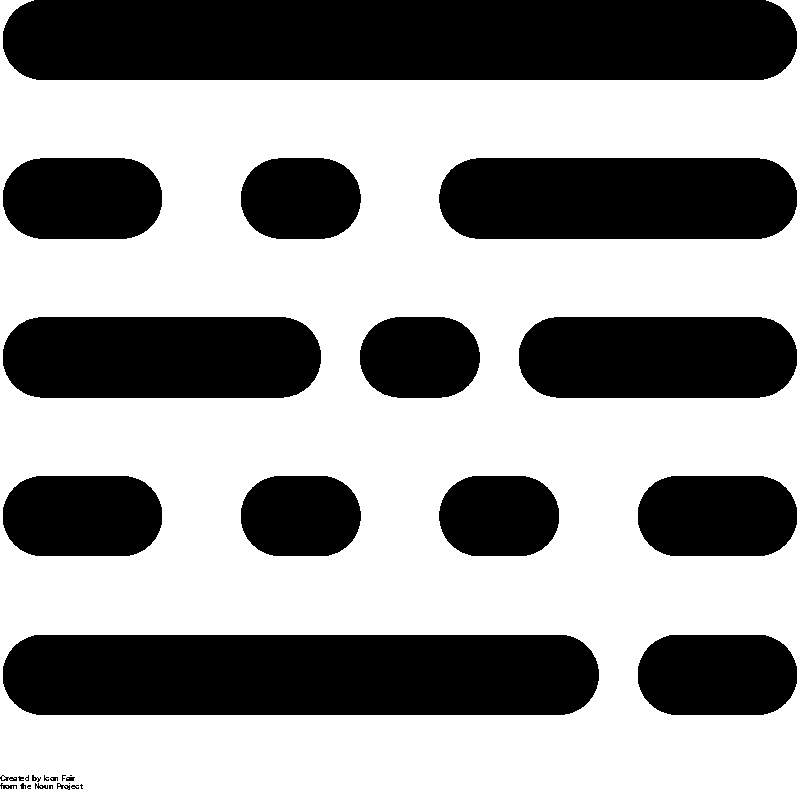
\includegraphics[trim=0mm 11mm 0 0,clip,scale=0.028,valign=c]{images/icons/text.pdf}}] Texts
% 	    \end{itemize}
% 	 \end{minipage}
%        }
%        \put (80,32) {
% 	 \begin{minipage}{0.1\textwidth}
% 	   Outputs
% 	 \end{minipage}
%        }
%       \end{overpic}
%     \end{minipage}
%     \begin{minipage}{\textwidth}
%       \centering
%       \begin{tabular}{c}
%         \phantom{text} \\
%         \phantom{text}
%       \end{tabular}
%     \end{minipage}
%   }
%
%   \only<2>{
%     \begin{minipage}{\textwidth}
%       \centering
%       \begin{overpic}[scale=0.4]{images/icons/neural_network_1.pdf}
%        \put (0,32) {
% 	 \begin{minipage}{0.3\textwidth}
% 	    \begin{itemize}
% 	      \item[{
\includegraphics[trim=4mm 11mm 0 0,clip,scale=0.2,valign=c]{images/icons/image.pdf}}] Images
% 	      \item[{
\includegraphics[trim=4mm 11mm 0 0,clip,scale=0.2,valign=c]{images/icons/sound.pdf}}] Sounds
% 	      \item[{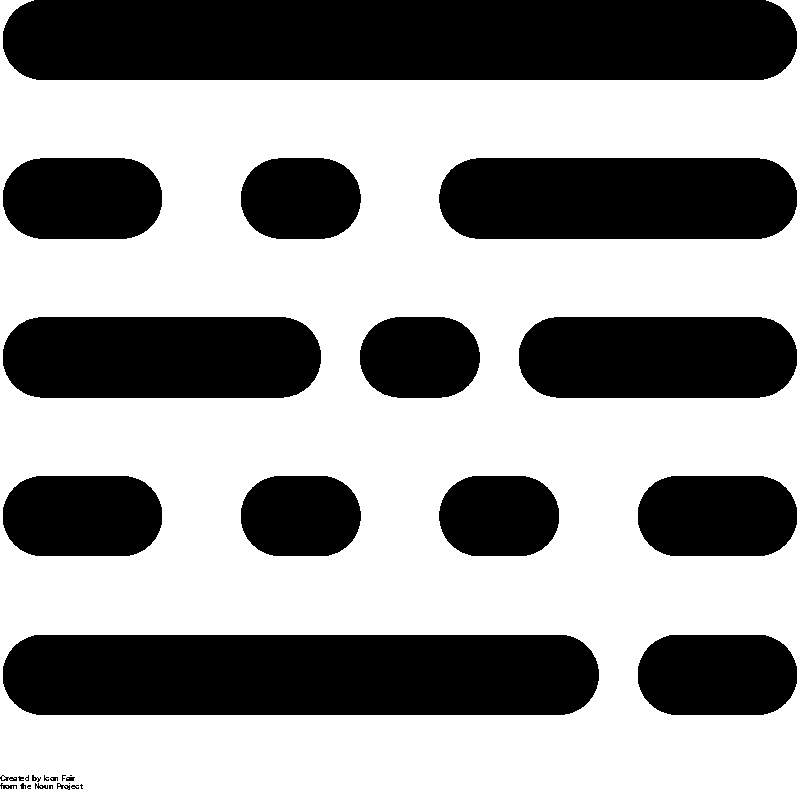
\includegraphics[trim=0mm 11mm 0 0,clip,scale=0.028,valign=c]{images/icons/text.pdf}}] Texts
% 	    \end{itemize}
% 	 \end{minipage}
%        }
%        \put (80,32) {
% 	 \begin{minipage}{0.1\textwidth}
% 	   Outputs
% 	 \end{minipage}
%        }
%        \put (41,19) {
% 	\begin{tikzpicture}
% 	  \draw[color=OrangePSL, thick] (0,0) -- (1.4,0) -- (1.4,2.5) -- (0,2.5) -- (0,0);
% 	\end{tikzpicture}
%        }
%        \put (45,49) {
%      \orangebold{Layer}
%        }
%       \end{overpic}
%     \end{minipage}
%     \begin{minipage}{\textwidth}
%       \centering
%       \begin{tabular}{c}
%         \phantom{text} \\
%         \phantom{text}
%       \end{tabular}
%     \end{minipage}
%   }
%
%   \only<3>{
%     \begin{minipage}{\textwidth}
%       \centering
%       \begin{overpic}[scale=0.4]{images/icons/neural_network_1.pdf}
%        \put (0,32) {
% 	 \begin{minipage}{0.3\textwidth}
% 	    \begin{itemize}
% 	      \item[{
\includegraphics[trim=4mm 11mm 0 0,clip,scale=0.2,valign=c]{images/icons/image.pdf}}] Images
% 	      \item[{
\includegraphics[trim=4mm 11mm 0 0,clip,scale=0.2,valign=c]{images/icons/sound.pdf}}] Sounds
% 	      \item[{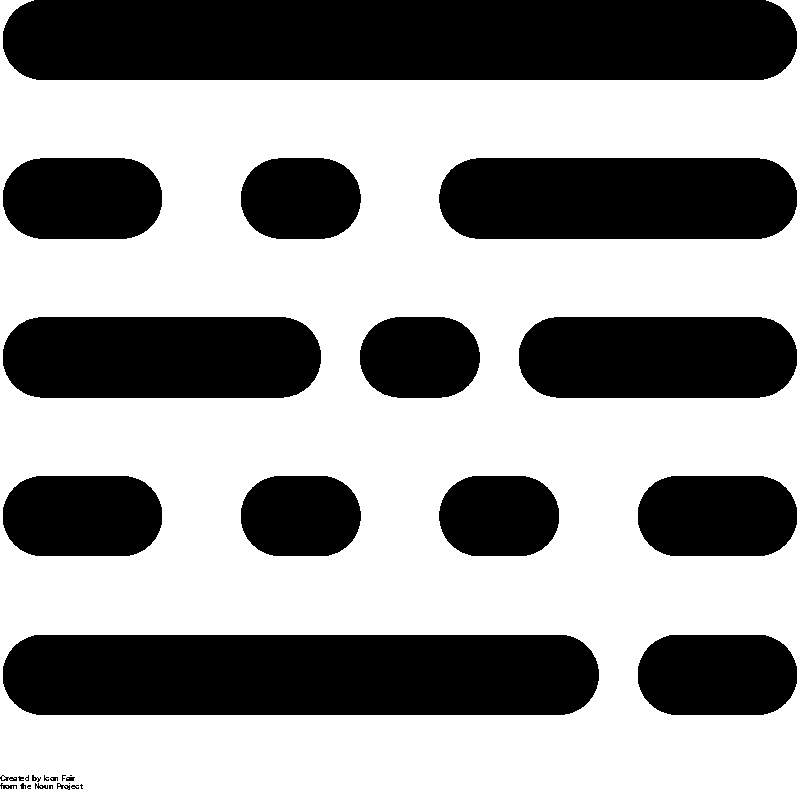
\includegraphics[trim=0mm 11mm 0 0,clip,scale=0.028,valign=c]{images/icons/text.pdf}}] Texts
% 	    \end{itemize}
% 	 \end{minipage}
%        }
%        \put (80,32) {
% 	 \begin{minipage}{0.1\textwidth}
% 	   Outputs
% 	 \end{minipage}
%        }
%        \put (52,41) {
% 	\begin{tikzpicture}
% 	    \draw[color=OrangePSL, thick, <-] (0,0) -- (0.8,0.5);
% 	\end{tikzpicture}
%        }
%        \put (51,35) {
% 	\begin{tikzpicture}
% 	  \draw[color=OrangePSL, thick, <-] (0,0) -- (0.9,1.0);
% 	\end{tikzpicture}
%        }
%        \put (50,26) {
% 	\begin{tikzpicture}
% 	    \draw[color=OrangePSL, thick, <-] (0,0) -- (1.0,1.7);
% 	\end{tikzpicture}
%        }
%        \put (62,45) {
%      \orangebold{Neurones}
%        }
%       \end{overpic}
%     \end{minipage}
%     \begin{minipage}{\textwidth}
%       \centering
%       \begin{tabular}{c}
%         In general, increasing the number of neurons makes the network more \\
%         \orangebold{expressive} and more \orangebold{accurate}.
%       \end{tabular}
%     \end{minipage}
%   }
%
%   \only<4>{
%     \begin{minipage}{\textwidth}
%       \centering
%       \begin{overpic}[scale=0.4]{images/icons/neural_network_2.pdf}
% 	\put (0,32) {
% 	 \begin{minipage}{0.3\textwidth}
% 	    \begin{itemize}
% 	      \item[{
\includegraphics[trim=4mm 11mm 0 0,clip,scale=0.2,valign=c]{images/icons/image.pdf}}] Images
% 	      \item[{
\includegraphics[trim=4mm 11mm 0 0,clip,scale=0.2,valign=c]{images/icons/sound.pdf}}] Sounds
% 	      \item[{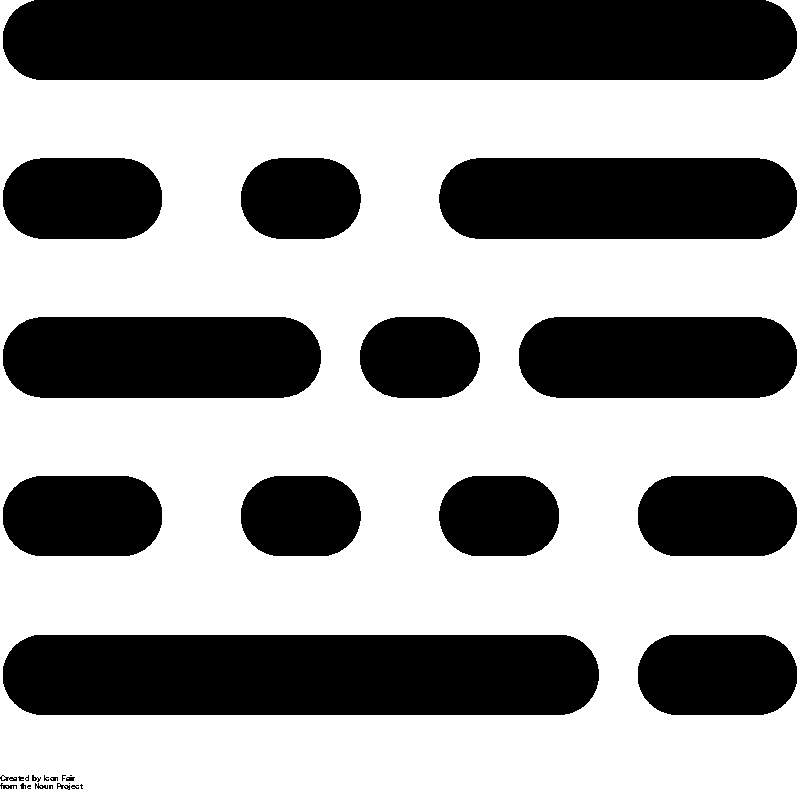
\includegraphics[trim=0mm 11mm 0 0,clip,scale=0.028,valign=c]{images/icons/text.pdf}}] Texts
% 	    \end{itemize}
% 	 \end{minipage}
%        }
%        \put (80,32) {
% 	 \begin{minipage}{0.1\textwidth}
% 	   Outputs
% 	 \end{minipage}
%        }
%       \end{overpic}
%     \end{minipage}
%     \begin{minipage}{\textwidth}
%       \centering
%       \begin{tabular}{c}
%         We can increase the number of neurons in each layer. \\
%         \phantom{text}
%       \end{tabular}
%     \end{minipage}
%   }
%   
%
%   \only<5>{
%     \begin{minipage}{\textwidth}
%       \centering
%       \begin{overpic}[scale=0.4]{images/icons/neural_network_3.pdf}
%        \put (0,32) {
% 	 \begin{minipage}{0.3\textwidth}
% 	    \begin{itemize}
% 	      \item[{
\includegraphics[trim=4mm 11mm 0 0,clip,scale=0.2,valign=c]{images/icons/image.pdf}}] Images
% 	      \item[{
\includegraphics[trim=4mm 11mm 0 0,clip,scale=0.2,valign=c]{images/icons/sound.pdf}}] Sounds
% 	      \item[{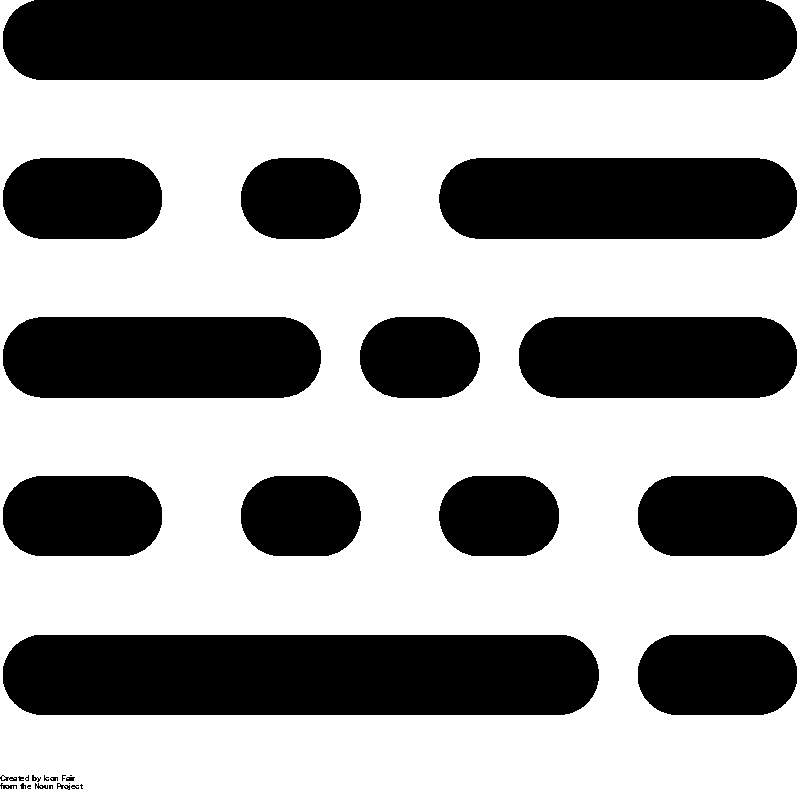
\includegraphics[trim=0mm 11mm 0 0,clip,scale=0.028,valign=c]{images/icons/text.pdf}}] Texts
% 	    \end{itemize}
% 	 \end{minipage}
%        }
%        \put (80,32) {
% 	 \begin{minipage}{0.1\textwidth}
% 	   Outputs
% 	 \end{minipage}
%        }
%       \end{overpic}
%     \end{minipage}
%     \begin{minipage}{\textwidth}
%       \centering
%       \begin{tabular}{c}
%         We can increase the number of neurons in each layer. \\
%         \phantom{text}
%       \end{tabular}
%     \end{minipage}
%   }
%
%
%   \only<6>{
%     \begin{minipage}{\textwidth}
%       \centering
%       \begin{overpic}[scale=0.4]{images/icons/neural_network_4.pdf}
%        \put (-10,32) {
% 	 \begin{minipage}{0.3\textwidth}
% 	    \begin{itemize}
% 	      \item[{
\includegraphics[trim=4mm 11mm 0 0,clip,scale=0.2,valign=c]{images/icons/image.pdf}}] Images
% 	      \item[{
\includegraphics[trim=4mm 11mm 0 0,clip,scale=0.2,valign=c]{images/icons/sound.pdf}}] Sounds
% 	      \item[{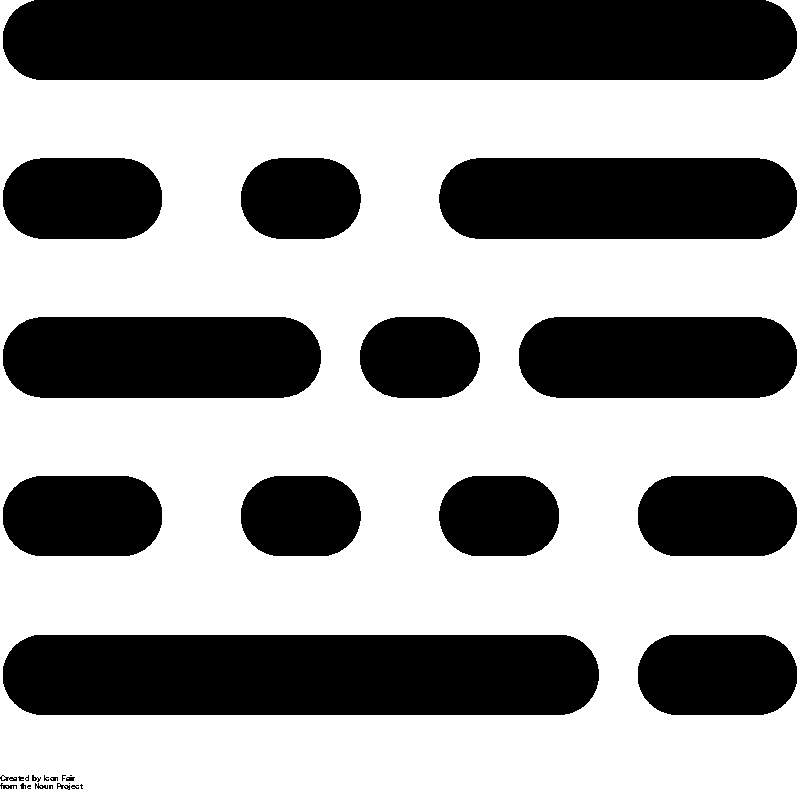
\includegraphics[trim=0mm 11mm 0 0,clip,scale=0.028,valign=c]{images/icons/text.pdf}}] Texts
% 	    \end{itemize}
% 	 \end{minipage}
%        }
%        \put (90,32) {
% 	 \begin{minipage}{0.1\textwidth}
% 	   Outputs
% 	 \end{minipage}
%        }
%       \end{overpic}
%     \end{minipage}
%     \begin{minipage}{\textwidth}
%       \centering
%       \begin{tabular}{c}
%         We can also increase the depth of Neural Networks by stacking more layers. \\
%         \phantom{text}
%       \end{tabular}
%     \end{minipage}
%   }
%
%
%   \only<7>{
%     \begin{minipage}{\textwidth}
%       \centering
%       \begin{overpic}[scale=0.4]{images/icons/neural_network_5.pdf}
%        \put (-15,32) {
% 	 \begin{minipage}{0.3\textwidth}
% 	    \begin{itemize}
% 	      \item[{
\includegraphics[trim=4mm 11mm 0 0,clip,scale=0.2,valign=c]{images/icons/image.pdf}}] Images
% 	      \item[{
\includegraphics[trim=4mm 11mm 0 0,clip,scale=0.2,valign=c]{images/icons/sound.pdf}}] Sounds
% 	      \item[{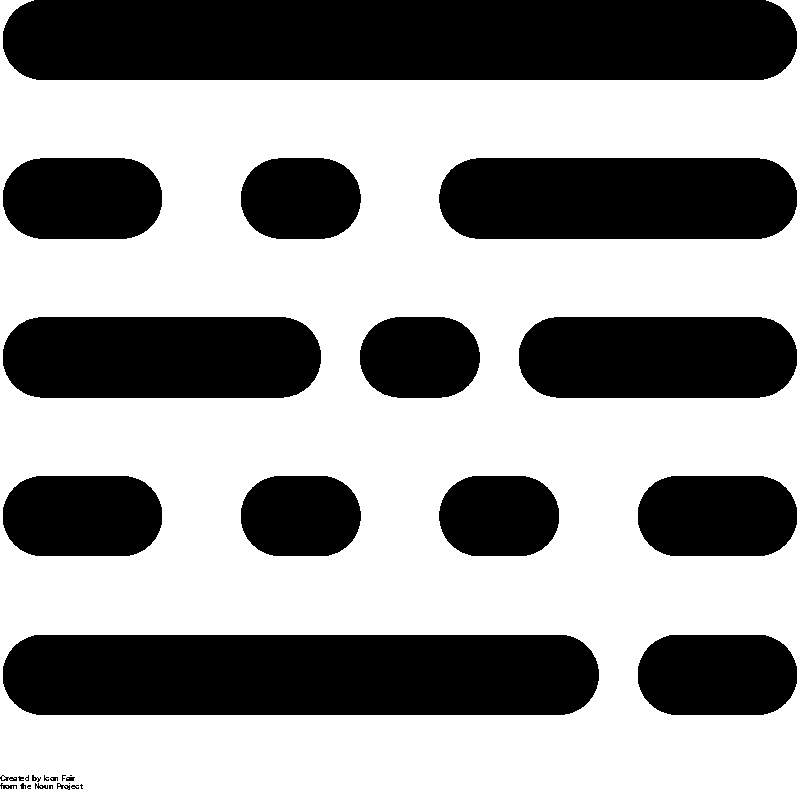
\includegraphics[trim=0mm 11mm 0 0,clip,scale=0.028,valign=c]{images/icons/text.pdf}}] Texts
% 	    \end{itemize}
% 	 \end{minipage}
%        }
%        \put (95,32) {
% 	 \begin{minipage}{0.1\textwidth}
% 	   Outputs
% 	 \end{minipage}
%        }
%       \end{overpic}
%     \end{minipage}
%     \begin{minipage}{\textwidth}
%       \centering
%       \begin{tabular}{c}
%         We can also increase the depth of Neural Networks by stacking more layers. \\
%         \phantom{text}
%       \end{tabular}
%     \end{minipage}
%   }
%
% \end{frame}



% %%%%%%%%%%%%%%%%%%%%%%%%%%%%%%%%%%%%%%%%%%%%%%%%%%%%%%%%%%%%%%%%%%%%%%%%%%%%%%%
% \begin{frame}{Limits of large Neural Networks}
% %%%%%%%%%%%%%%%%%%%%%%%%%%%%%%%%%%%%%%%%%%%%%%%%%%%%%%%%%%%%%%%%%%%%%%%%%%%%%%%
%
%   \begin{minipage}{\textwidth}
%     \centering
%     Large Neural Networks are \orangebold{accurate} but have several \orangebold{drawbacks}.
%   \end{minipage}
%
%   \begin{minipage}{\textwidth}
%     \centering
%     \begin{tikzpicture}
%       \draw[color=white, ->, thick, onslide=<2->{color=OrangePSL}] (0,0) -- (-2.1,-0.6);
%       \draw[color=white, ->, thick, onslide=<3->{color=OrangePSL}] (0,0) -- (+2.1,-0.6);
%     \end{tikzpicture}
%   \end{minipage}
%
%   \begin{minipage}{0.49\textwidth}
%     \centering
%     \visible<2->{
%       
\includegraphics[scale=0.05]{./images/icons/data-center.pdf} \\
%       \footnotesize{Computationally \\ Expensive}
%     }
%   \end{minipage}
%   \begin{minipage}{0.49\textwidth}
%     \centering
%     \visible<3->{
%       
\includegraphics[scale=0.05]{./images/icons/hacker.pdf} \\
%       \footnotesize{Vulnerable to \\ adversarial attacks}
%     }
%   \end{minipage}
%   \vspace{0.5cm}
%   
%
%   \visible<4->{
%     \begin{mdframed}[linecolor=OrangePSL,linewidth=1pt]
%       \centering
%       The evaluation of Neural Networks should be \orangebold{multi-criteria}.
%     \end{mdframed}
%   }
%
%   \visible<5->{
%     \begin{block}{Neural Networks should ...}
%       \begin{itemize}
% 	\item[$\bullet$] maximize the accuracy;
% 	\item[$\bullet$] have a small numbers of parameters;
% 	\item[$\bullet$] be robust against adversarial attacks.
%       \end{itemize}
%     \end{block}
%   }
%
% \end{frame}





% %%%%%%%%%%%%%%%%%%%%%%%%%%%%%%%%%%%%%%%%%%%%%%%%%%%%%%%%%%%%%%%%%%%%%%%%%%%%%%%%
% \begin{frame}{Examples self-driving cars}
% %%%%%%%%%%%%%%%%%%%%%%%%%%%%%%%%%%%%%%%%%%%%%%%%%%%%%%%%%%%%%%%%%%%%%%%%%%%%%%%%
%
%   \begin{minipage}{\textwidth}
%     \centering
%       \begin{minipage}{0.2\textwidth}
% 	\includegraphics<1>[scale=0.05]{images/stop_sign.pdf}
% 	\includegraphics<2->[scale=0.05]{images/stop_sign_adv.pdf}
%       \end{minipage}
%       \begin{minipage}{0.3\textwidth}
% 	\includegraphics<1>[trim=1.5cm 4cm 1.8cm 5cm,clip,scale=0.4]{images/car.pdf}
% 	\includegraphics<2->[trim=1.5cm 4cm 1.8cm 5cm,clip,scale=0.4]{images/car_signal.pdf}
%       \end{minipage}
%   \end{minipage}
%
% \end{frame}








% %%%%%%%%%%%%%%%%%%%%%%%%%%%%%%%%%%%%%%%%%%%%%%%%%%%%%%%%%%%%%%%%%%%%%%%%%%%%%%%
% \begin{frame}{Feedfoward Neural Networks}
% %%%%%%%%%%%%%%%%%%%%%%%%%%%%%%%%%%%%%%%%%%%%%%%%%%%%%%%%%%%%%%%%%%%%%%%%%%%%%%%
%
%   A Neural Neural can be analytically described as a composition of linear functions interlaced with non-linear functions:
%   \vspace{0.2cm}
%   \begin{equation}
%     N_\Omega(\xvec) = \phi^{(p)} \circ \phi^{(p-1)} \circ \cdots \circ \phi^{(1)}(\xvec)
%   \end{equation}
%   where each layer is defined:
%   $\phi^{(i)} \triangleq \xvec \mapsto 
%     {\color<2>{OrangePSL}{\rho \big(}}
%     \ {\color<3>{OrangePSL}{\Wmat^{(i)}}} \xvec + {\color<3>{OrangePSL}{\bvec^{(i)}}} \ 
%     {\color<2>{OrangePSL}{\big)}}$
%
%   {\beamerdefaultoverlayspecification{<+->}
%     \begin{itemize}
%       \item 
%       \item[$\bullet$] $\rho$ is a non linear function (\eg, ReLU, Leaky-ReLU, Sigmoid, etc.)
%       \item[$\bullet$] $\Wmat^{(i)}$ is a $n \times n$ matrix and $\bvec^{(i)}$ is a vector of size $n$ are the parameters.
%     \end{itemize}
%   }
%
%   \vspace{0.5cm}
%   \visible<4>{
%     \begin{mdframed}[linecolor=OrangePSL,linewidth=1pt]
%       \centering
%       For fixed width $n$, the network will have $p n (n + 1)$ parameters.
%     \end{mdframed}
%   }
%
% \end{frame}



% %%%%%%%%%%%%%%%%%%%%%%%%%%%%%%%%%%%%%%%%%%%%%%%%%%%%%%%%%%%%%%%%%%%%%%%%%%%%%%%
% \begin{frame}{Convolutional Neural Networks}
% %%%%%%%%%%%%%%%%%%%%%%%%%%%%%%%%%%%%%%%%%%%%%%%%%%%%%%%%%%%%%%%%%%%%%%%%%%%%%%%
%
%   \begin{minipage}{\textwidth}
%     \centering
%     Convolutional Neural Networks are state-of-the-art for image classification.
%   \end{minipage}
%   \vspace{0.2cm}
%
%   \begin{minipage}{\textwidth}
%     \centering
%       \includegraphics[trim=1cm 1.8cm 1.3cm 0, clip, scale=0.35]{FCN32/main.pdf}
%     \\ 
%     \footnotesize{Convolutional Neural Network Architecture}
%   \end{minipage}
%
%   \vspace{0.5cm}
%   \pause
%   \begin{minipage}{\textwidth}
%     \centering
%     Convolutional Neural Networks are a specific type \\ of \orangebold{structured neural networks}.
%     % Convolutional Neural Networks use a specific \orangebold{structure as linear operations}. 
%   \end{minipage}
%
% \end{frame}



